% !TEX root = ../../report.tex

\section{Data Findings}
\subsection{What Can Be Understood From The Data}

%Dataset summary
    %How many users?
    %How much preference data?
    %Which events are interesting to look at?


\subsubsection{The Expected}
Event "app\_started", all have user\_id's
Event "app\_first\_started", all user\_id's are NULL
Event "user\_logged\_in", all have user\_id's... (assigned with login, event saved after login?)

\subsubsection{The Strange}
NULL valued  for user\_id events: (Not all strange, but put together for readability)
facebook\_share\_changed

collection\_viewed  ignoring collection view-event as of now since the user\_id
is null. Could be valuable to use, though (30 000 events ignored) ...
potential workaround:
    for each session do:
        Filter all events on:
            session-ts-start to session-ts-end,
            allow: user\_id session-user-id and NULL
            Ip of user-session and ip of collection\_viewed
            storefront\_id's from session
                Populate collection\_viewed-user-id with session-user-id

Potential faulty user-id setting for ip-switch during a session, but expect few
occurrences of this

wantlist\_menu\_entry\_clicked
app\_became\_active

app\_first\_started
facebook\_login\_failed

> db.prod.distinct('event\_json.ipAddress').length
9033
> db.prod.distinct('event\_json.eventData.device\_id').length
2644
> db.prod.distinct('user\_id').length
1660

More devices than users, can't fill the blanks with device\_id

Q's:
    app\_became\_active id's for better sessions?
    store\_clicked vs. storefront\_clicked (23 vs. 19744)
    API item-id's mapping to event product\_id's; how to map?



soBazar want to build a proper model.  Give input on how to build this model.
The supplier should know that an item is a jacket for instance.  Have something
to show on the 20. Should be better than what is already implemented.



\subsection{Graphs}

Interesting fields from data:

    Events: userid - prodid - storeid - time - price? - applicationstate - (eventlocation)

    Offer: prodid - price(old/new) - storeid -time -

Thoughts on graphs (some of these will be in the appendix/removed, placed here
for simplicity and structure) (event database filtered on "server-environment"
with "prod" as value and removed all events with "simulator" as "platform"):



    Simple:

\begin{table}[H]
    \centering
    \begin{tabular}{l|l|l}
    ~                  & Amount & Notes                                  \\ \hline
    Unique users       & 1658   & Count of unique users in eventdatabase \\ \hline
    Unique item names  & 2591   & > db.prod.distinct('product\_name').length \\ \hline
    Unique item ids    & 4042   & > db.prod.distinct('product\_id').length TODO, remove one?  \\ \hline
    Unique brands      & 15     & > db.offer.distinct('brandId').length \tablefootnote{Count stores unique (not collections, but from offer (the items database) db)  (The missing 4 (the last two are null and N/A). These are foreign brands i.e. unknown, maybe test brands. 45002,38002,44004,55006)} \\ \hline
    Unique storefronts & 21     & > db.prod.distinct('retailer\_brand').lengthCount stores unique (from prod db)     \\
    \end{tabular}
\end{table}


\begin{table}[H]
    \centering
    \begin{tabular}{l|l|l}
        NonMatching values:           & 620    & ~ \\ \hline
        Offer database length         & 7854   & ~ \\ \hline
        Event items length           & 4042   & ~ \\ \hline
        Items from list2 not in list1 & 7.89 \% & ~ \\
    \end{tabular}
    \caption { Items in events not in the actual offer database }
\end{table}

        Price ranges of all items (groupings)

\begin{figure}[H]
    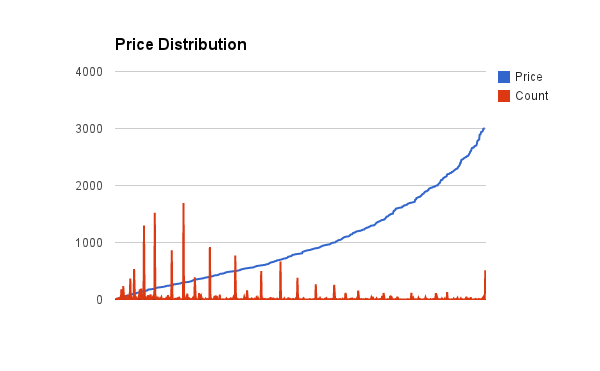
\includegraphics[width=5in]{image/price_distr.png}
    \centering
    \caption[Price distribution of items]{some awesome text}
    \label{figure:ratingdistr}
\end{figure}

        (Distinct event locations)TODO

        Item time on market TODO maybe not that interesting alone


    complex 2.Deg:

        Count for different events

\begin{figure}[H]
    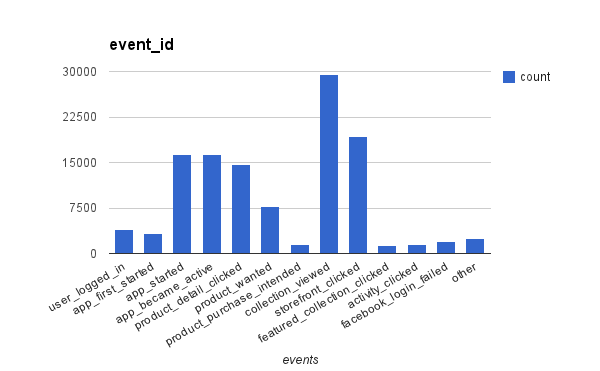
\includegraphics[width=5in]{image/event_id.png}
    \centering
    \caption[Count for different events]{some awesome text}
\end{figure}

        Distinct events done on stores (shady)

\begin{figure}[H]
    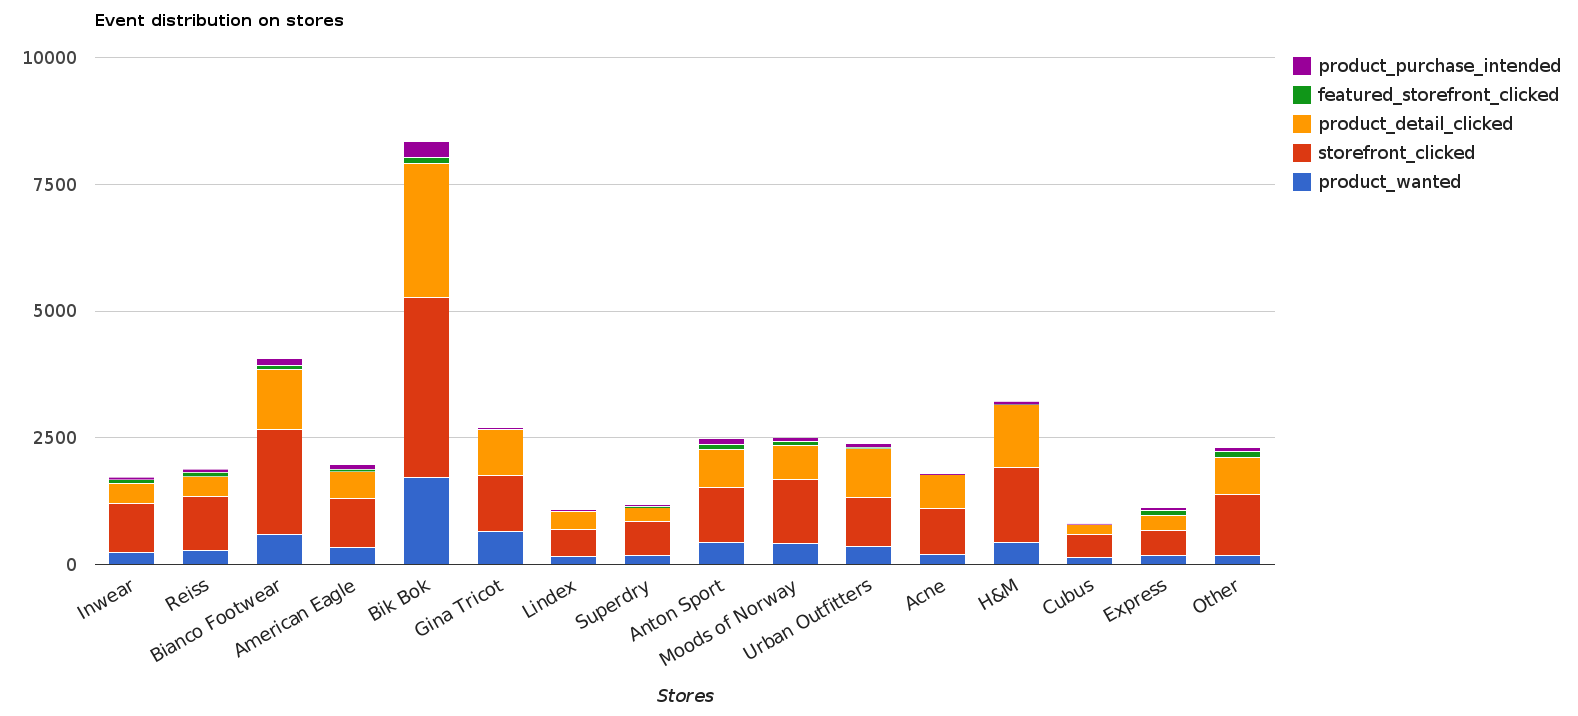
\includegraphics[width=5in]{image/event_distr.png}
    \centering
    \caption[Distribution of events on storefronts]{some awesome text}
\end{figure}

\begin{figure}[H]
    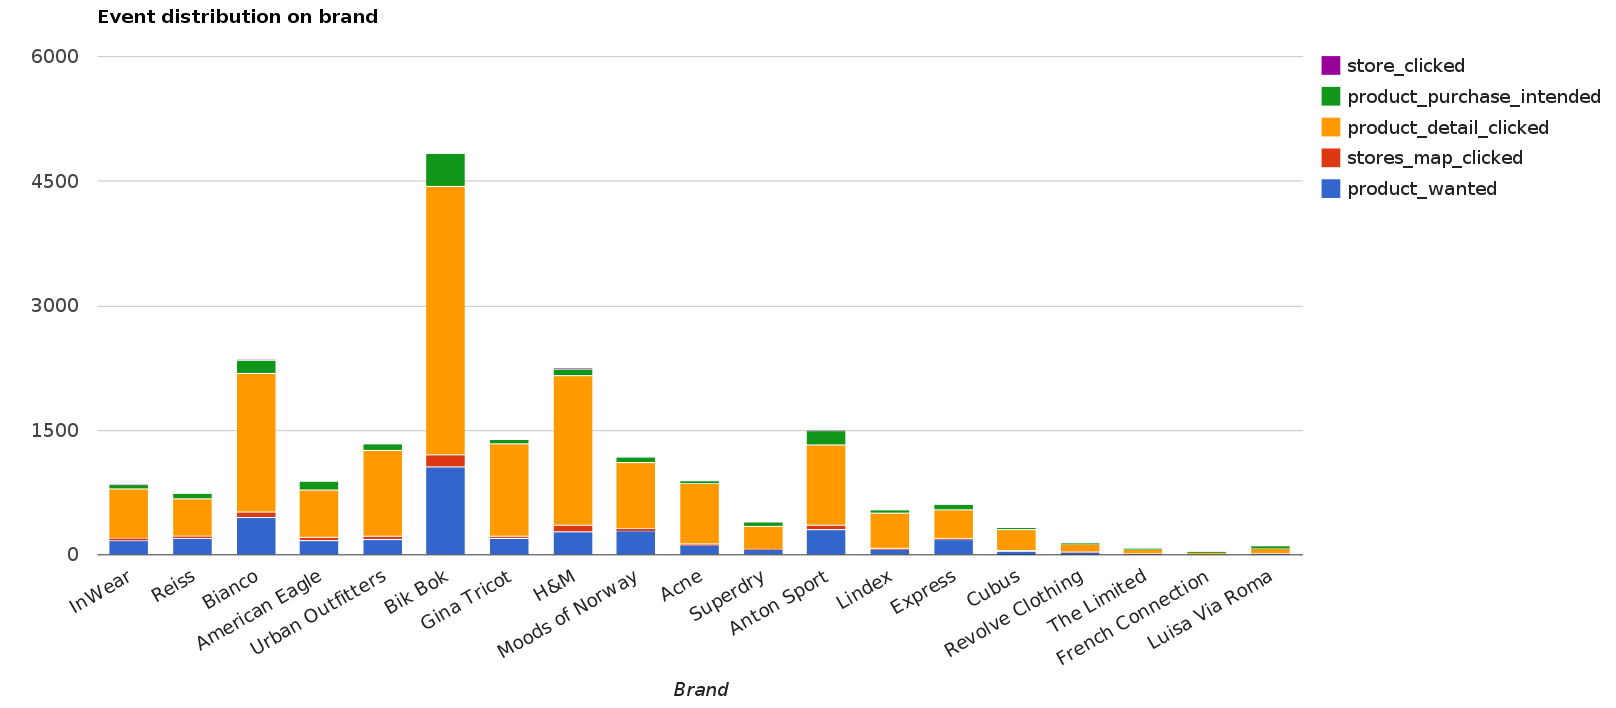
\includegraphics[width=5in]{image/brand_distr.png}
    \centering
    \caption[Distribution of events on brands]{some awesome text}
\end{figure}

        peak online (slope-style) (events per day)

\begin{figure}[H]
    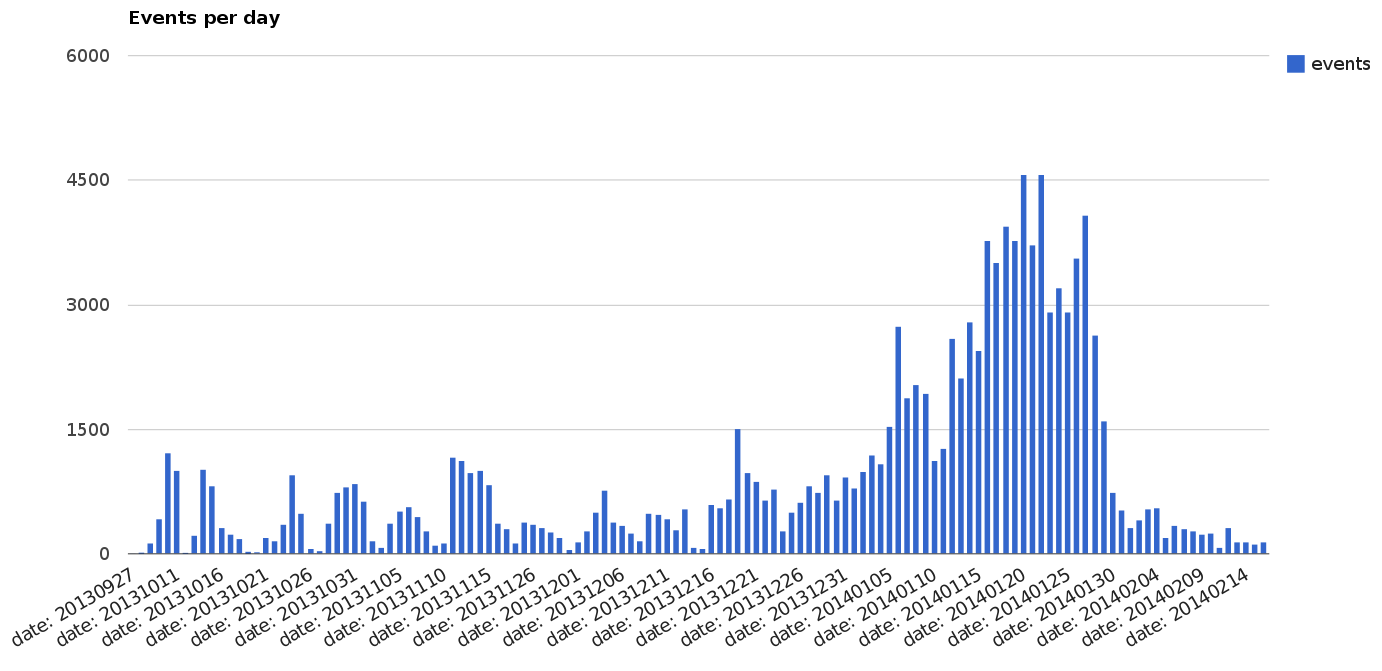
\includegraphics[width=5in]{image/events_per_day.png}
    \centering
    \caption[Distribution of events per day]{TODOsome awesome text}
\end{figure}


        Price range of items in stores



        count User eventes
        user-item (how many items has a user "interacted" with)
        Count of unique items in item db also in event db
        Usable events regarding userid (events types with not null userid)
        (Plotting locations)

\begin{figure}[H]
    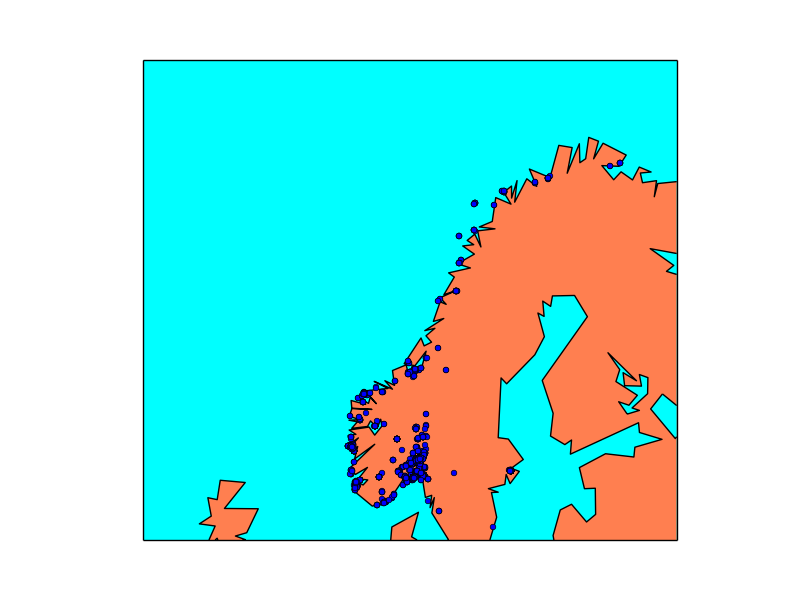
\includegraphics[width=5in]{image/simpleGeoPlot.png}
    \centering
    \caption[Simple plotting of event location]{TODOsome awesome text}
\end{figure}


        unique Stores count for users

    complex 3.Deg:

        count Sessions for users (aprox: sessioncount)TODO

\begin{figure}[H]
    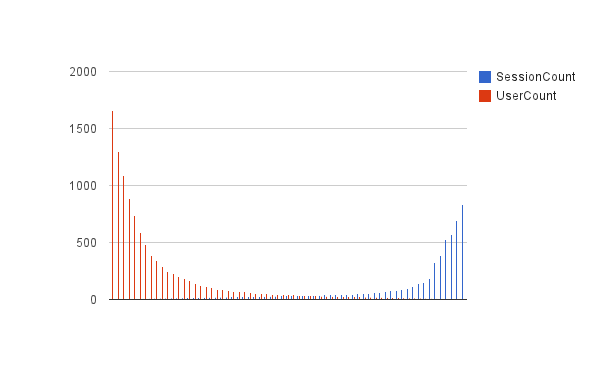
\includegraphics[width=5in]{image/global_sessioncount.png}
    \centering
    \caption[Count of sessions per user mapped with count of user with give
    session amount]{TODOsome awesome text}
\end{figure}

        price span for user

    complex 4.Deg:

        Stats for sessions:

            Timespann of sessions for users (avg, max, min)
            Events per session (avg, max, min)
            Item viewtime for user in session
            Stores visited per session
            revisit time of items for user
            relationship with view, want and purchase
            time of session over lifetime of app
            user preferred price in session

    complex 5.Deg:

        Stats for global session stats:

            price vs view, want and purchase
            avg viewtime for an item (i know)
            Similarity of user favorite store, items viewed and items wanted?
            time of session over lifetime of app for all users (slope-style)

    complex 6.Deg:

TODO: STRUCTURExfdgdsagCFG
SDFG

    Blobs of smaller bubbles with eventid
    Blobs for eventcount on stores with items items from stores (populate "storename" for "itemevents")
    Show occurence of event after other event?
    User stats: items, likes, intented purchased, events, session avg, max event, fequency
    Find prices for stores: prize ranges
    User

Visuals:
    BubbleChart

To be done to 17:
    - PP
    - List articles to be read
    - Prototype implementation
    - Research question(s)
    -

New for 20.:
    - Make some awesome slides
    - scalable
    - collaborative filtering
    - somethingsomething
    - some architecture?
